% \textbf{Application of PLS-SEM} 

% Having developed the constructs and hypotheses, we will now apply PLS-SEM to analyze the data collected from the responses to questions 4-10. This analysis will involve the following steps: 

% \textbf{1. Model Specification:} 

% Define the relationships between constructs and indicators. Specify the hypothesized relationships among the constructs. 

% \textbf{2. Data Collection and Preparation:} 

% Gather responses to the selected questions. Prepare the data for analysis, ensuring it meets the requirements for PLS-SEM. 

% \textbf{3. Model Estimation:} 

% Use PLS-SEM software to estimate the model parameters. Assess the measurement model for reliability and validity. 

% \textbf{4. Structural Model Evaluation:} 

% Evaluate the structural model by examining path coefficients and the significance of hypothesized relationships. Assess the model’s explanatory power through measures such as R-squared and Q-squared statistics. 

% \textbf{5. Hypothesis Testing: }

 

% Test the formulated hypotheses using the results from the structural model evaluation. Validate or invalidate each hypothesis based on the significance and direction of the relationships. Through this systematic application of PLS-SEM, we aim to derive meaningful insights from our data and validate the proposed hypotheses, thereby advancing our understanding of the impact of pandemic disruptions on change management and resilience strategies. 

\subsection{Application of PLS-SEM}

In our study, we utilized SmartPLS 4 \parencite{smartpls2024} to analyze the structural equation model (SEM) based on the survey data collected. The constructs and hypotheses were operationalized through a series of survey questions, each carefully designed to measure specific aspects of the constructs in question. Below, we will elaborate on the process of model construction and the rationale behind the arrows and dependencies depicted in the Figure \ref{fig:constructs}. The survey data comprised questions targeted at measuring three main constructs: Pandemic Disruption, Change Management, and Resilience Effectiveness. Each of these constructs was associated with specific questions from the survey. For Pandemic Disruption, we used Question 4 which assesses the extent to which companies experienced supply chain disruptions due to the pandemic. This question serves as a critical indicator of the impact of COVID-19 on operational stability. Change Management was measured using Questions 5, 6, 8, 9, and 10. These questions capture various strategic responses implemented during the pandemic, including changes in supply management strategies, supplier diversification, creation of backup plans, adjustment of demand forecasting methods, and the presence of formal pandemic preparedness plans. These aspects collectively reflect the strategic adaptability and preparedness measures undertaken by companies in response to the pandemic. Resilience Effectiveness was gauged through Question 7, which evaluates the effectiveness of the company's resilience strategies such as inventory management and supplier diversification during the pandemic. This construct provides insights into how well existing strategies mitigated the pandemic's impact. The diagram also incorporates the specific survey questions associated with each construct, denoted by the yellow text boxes. For example, CMQ10, CMQ5, CMQ6, CMQ8, and CMQ9 represent the questions related to Change Management. The arrows pointing towards the Change Management node indicate the reflective measurement model, where each question (indicator) is influenced by the underlying construct. PLS-SEM analysis is well suited for various types of research data, some of them being the Likert Scale, which typically is a 5-point scale where respondents indicate their level of agreement or disagreement with a statement. The scales usually range from "Strongly Agree" to "Strongly Disagree", or similar. Likert scales are popular in measuring attitudes, perceptions, and behavioral intentions. It is also suited for Binary or Dichotomous Scales, which are simple yes/no or true/false responses. In our case, the responses for Questions 4 and 7 are in the Likert Scale and the responses for Questions 5, 6, 8, 9 and 10 are within the Binary Scale. This is briefly below.

\subsubsection{Methodology Steps}

\paragraph*{Selection of Questions for Analysis:} To apply PLS-SEM, we selected questions 4 to 10 for analysis. These questions were chosen because they are either yes/no questions or questions with answers on a scale ranging from 0 to 5, which are suitable for the PLS-SEM modeling approach.

\paragraph*{Construct Development:} To create meaningful hypotheses, constructs are developed based on the questions asked, specifically questions 4-10. Constructs represent the theoretical concepts that underpin the variables of interest in the study.

\paragraph*{Hypothesis Creation and Validation:} The primary objective is to formulate hypotheses based on the research questions and subsequently validate or invalidate them using the responses received. The validation will be conducted through the results obtained from the PLS-SEM analysis.

\paragraph*{Summary of Process:}

\begin{itemize}
    \item \textbf{Step 1:} Select objective questions (Questions 4-10).
    \item \textbf{Step 2:} Develop constructs based on the selected questions.
    \item \textbf{Step 3:} Formulate hypotheses related to the developed constructs.
    \item \textbf{Step 4:} Apply PLS-SEM to analyze the data and obtain results.
    \item \textbf{Step 5:} Validate or invalidate the hypotheses based on the analysis results.
\end{itemize}

\subsubsection{Constructs Developed}

\paragraph*{Construct 1: Pandemic Disruption}

\begin{itemize}
    \item \textbf{Question Used:} Question 4
    \item This construct is based on a question that measures the extent to which companies experienced disruption in their supply chain due to the pandemic. It serves as an indicator of the overall impact of COVID-19 on operations.
\end{itemize}

\paragraph*{Construct 2: Change Management}

\begin{itemize}
    \item \textbf{Questions Used:} Questions 5, 6, 8, 9, 10
    \item These questions pertain to various changes implemented in response to the pandemic, including adjusting management strategies, diversifying suppliers, creating backup plans, adjusting forecasting methods, and formalizing preparedness plans. These questions reflect the strategic adaptability and preparedness measures taken by companies.
\end{itemize}

\paragraph*{Construct 3: Resilience Effectiveness}

\begin{itemize}
    \item \textbf{Question Used:} Question 7
    \item This construct evaluates the effectiveness of the company’s resilience strategies during the pandemic, such as inventory management and supplier diversification.
\end{itemize}



\begin{figure}[H]
  \centering
  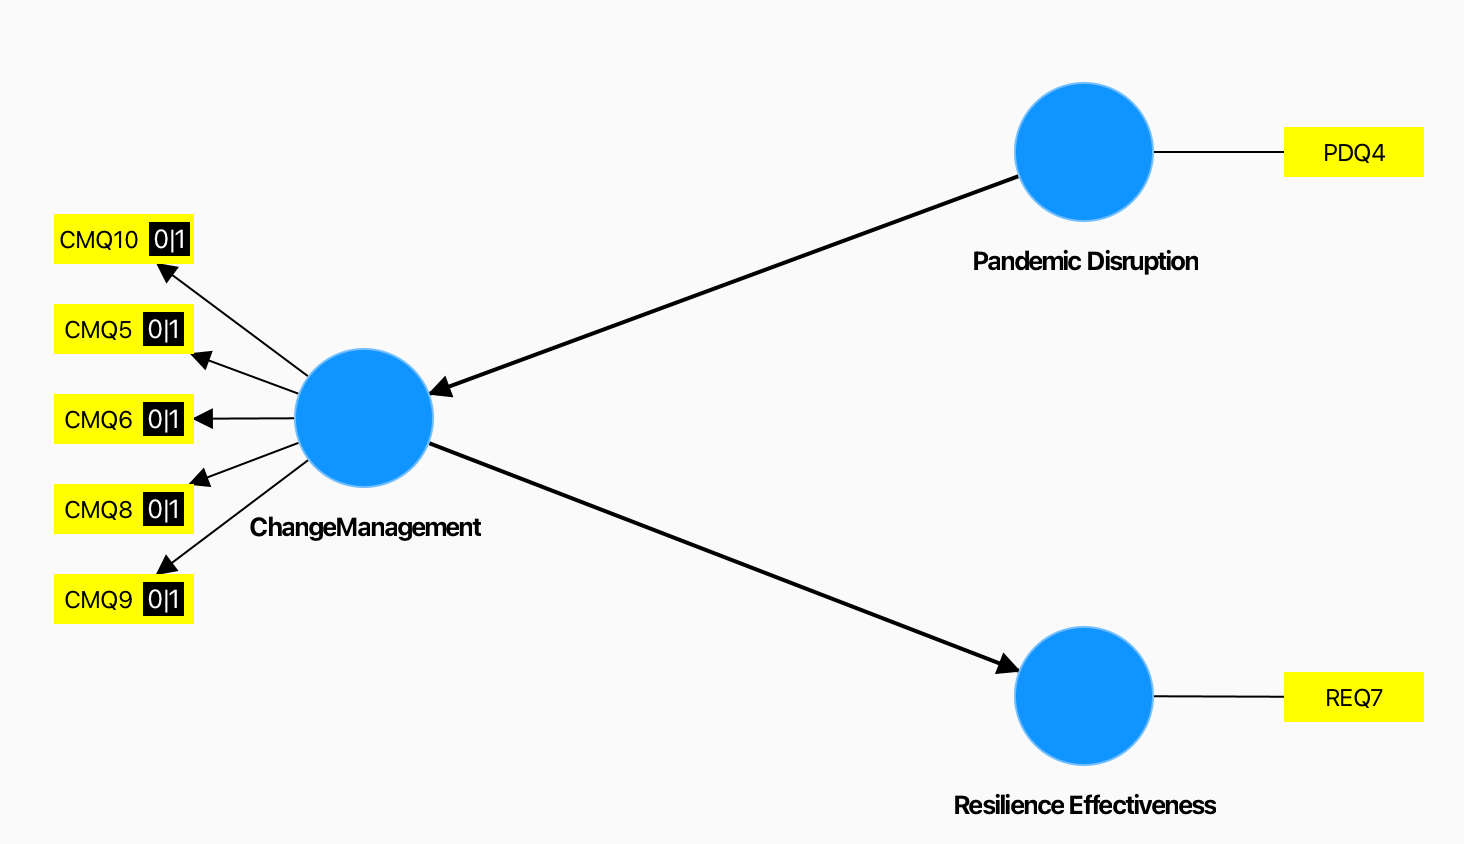
\includegraphics[width=1\textwidth]{figure/initial_model.png}
  \caption{Structural Model in SmartPLS showing the relationships between constructs. The model includes Pandemic Disruption (Q4), Change Management (Q5, Q6, Q8, Q9, 10), and Resilience Effectiveness (Q7). Arrows indicate hypothesized dependencies: Pandemic Disruption's impact on Change Management and Resilience Effectiveness, and Resilience Effectiveness's influence on Change Management. $[0|1]$ Adjacent to the question numbers indicate the binary nature of the questions. Other questions belong to the Likert Scale.}
  \label{fig:constructs}
\end{figure}


Using SmartPLS 4, we constructed a model (Figure \ref{fig:constructs}) to test our hypotheses. The structural model posits the following relationships:

\begin{enumerate}
    \item \textbf{Pandemic Disruption leads to Change Management (H1)}: This hypothesis suggests that higher levels of disruption due to the pandemic are positively associated with an increase in change management strategies. The arrow from Pandemic Disruption to Change Management in the diagram represents this hypothesis. The rationale is that significant disruptions necessitate strategic changes to adapt and mitigate the impact.

    \item \textbf{Resilience Effectiveness reduces the need for extensive Change Management (H2)}: This hypothesis proposes a negative relationship between the effectiveness of resilience strategies and the extent of change management. If a company’s existing resilience strategies are effective, it may not need to implement extensive changes. This is depicted by the arrow from Resilience Effectiveness to Change Management, indicating that effective resilience strategies can mitigate the need for further change.

    \item \textbf{Pandemic Disruption influences Resilience Effectiveness (H3)}: This hypothesis posits a positive relationship between the level of pandemic disruption and the perceived effectiveness of resilience strategies. Higher levels of disruption may prompt companies to evaluate and enhance their resilience strategies, thus leading to higher effectiveness. This relationship is shown by the arrow from Pandemic Disruption to Resilience Effectiveness in the diagram.

\end{enumerate}

Upon conducting the analysis using the SmartPLS tool for PLS-SEM, we can evaluate the validity of our hypothesized relationships among the constructs. By examining the path coefficients, significance levels (p-values), and the R² values for each endogenous construct, SmartPLS provides comprehensive insights into the strength and significance of the proposed causal paths. In our specific case, this involves assessing whether the hypothesized positive relationship between Pandemic Disruption and Change Management, the negative relationship between Resilience Effectiveness and Change Management, and the positive relationship between Pandemic Disruption and Resilience Effectiveness hold true. Additionally, the bootstrapping procedure available in SmartPLS allows us to obtain estimates of standard errors and confidence intervals, further solidifying our hypothesis testing. The evaluation of the model fit indices, such as the SRMR (Standardized Root Mean Square Residual), will help determine the overall adequacy of our model, enabling us to conclude whether the empirical data supports our theoretical propositions. Thus, the detailed results obtained from SmartPLS will enable us to confirm or refute our hypotheses with a considerable degree of statistical confidence. In configuring the SmartPLS software for our PLS-SEM analysis, several key settings were chosen to ensure interpretable results. We selected the Principal Component Analysis (PCA) weighting scheme, a common default choice, as it uses the first principal component of the block’s indicators as the composite score, providing a reliable and standard approach. To facilitate easier interpretation of path coefficients and enable comparisons across constructs, we opted for standardized results, which convert all variables to a common scale. For the initial weights, we adhered to the algorithm’s default settings. Regarding the handling of missing values, considering that only one response was partially missing, we utilized casewise deletion, provided it did not significantly reduce our sample size below acceptable limits for robust analysis. Lastly, we did not apply any additional weighting vectors, as none were necessary for our analysis.

\subsection{Results and Analysis of PLS-SEM}

\begin{figure}[h]
  \centering
  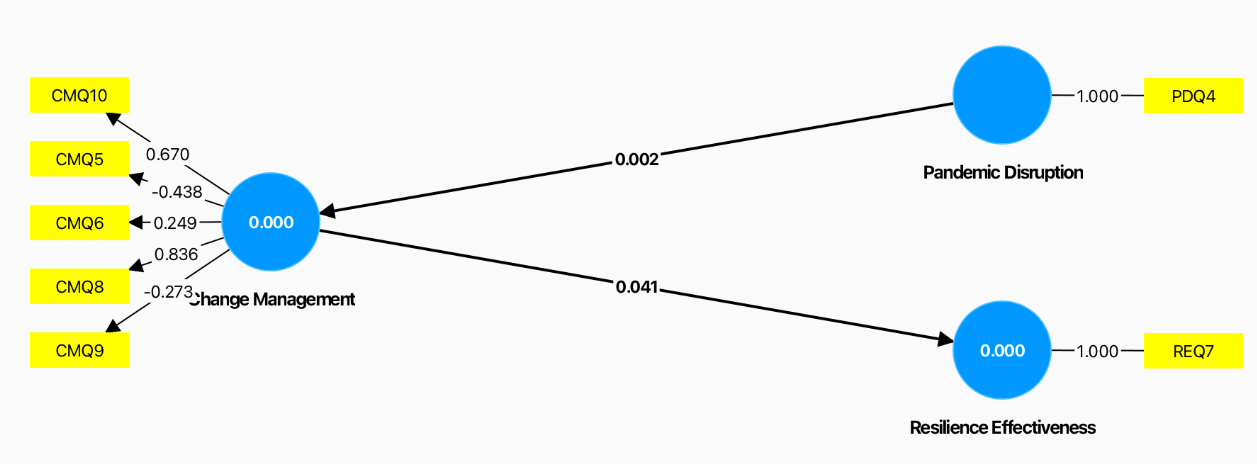
\includegraphics[width=1\textwidth]{figure/pls_sem_results_cropped.png}
  \caption{PLS-SEM Results showcasing path coefficients between constructs.}
  \label{fig:pls_sem_results}
\end{figure}

The results of our PLS-SEM analysis, depicted in Figure \ref{fig:pls_sem_results}, reveal the path coefficients among the constructs of Pandemic Disruption, Change Management, and Resilience Effectiveness. The path coefficient from Pandemic Disruption to Change Management is 0.002, suggesting a minimal positive influence of pandemic-induced disruptions on the extent of change management strategies implemented. This indicates that while pandemic disruptions might necessitate some strategic changes, the direct impact observed here is negligible. Conversely, the path coefficient from Resilience Effectiveness to Change Management is 0.041, implying a slight positive relationship. This suggests that as the effectiveness of resilience strategies increases, there is a marginal but positive impact on change management practices, indicating that companies with effective resilience strategies may still engage in proactive change management. The negative coefficients observed within the Change Management construct, such as -0.438 for CMQ5, -0.249 for CMQ6, and -0.273 for CMQ9, indicate that these specific aspects of change management may inversely relate to the overall construct. This could mean that certain change management practices, possibly those perceived as less effective or unnecessary, might detract from the overall strategic change efforts. The positive coefficients, such as 0.670 for CMQ10 and 0.836 for CMQ8, highlight the aspects that contribute positively to Change Management, signifying effective practices that enhance strategic adaptability. The significant values of 1.000 for PDQ4 and REQ7 indicate strong relationships of these specific questions with their respective constructs, emphasizing their reliability as indicators. Following the discussion on the path coefficients and their implications, we now turn our attention to additional metrics and validity assessments to provide further analysis of the model's performance.

\begin{figure}[h]
  \centering
  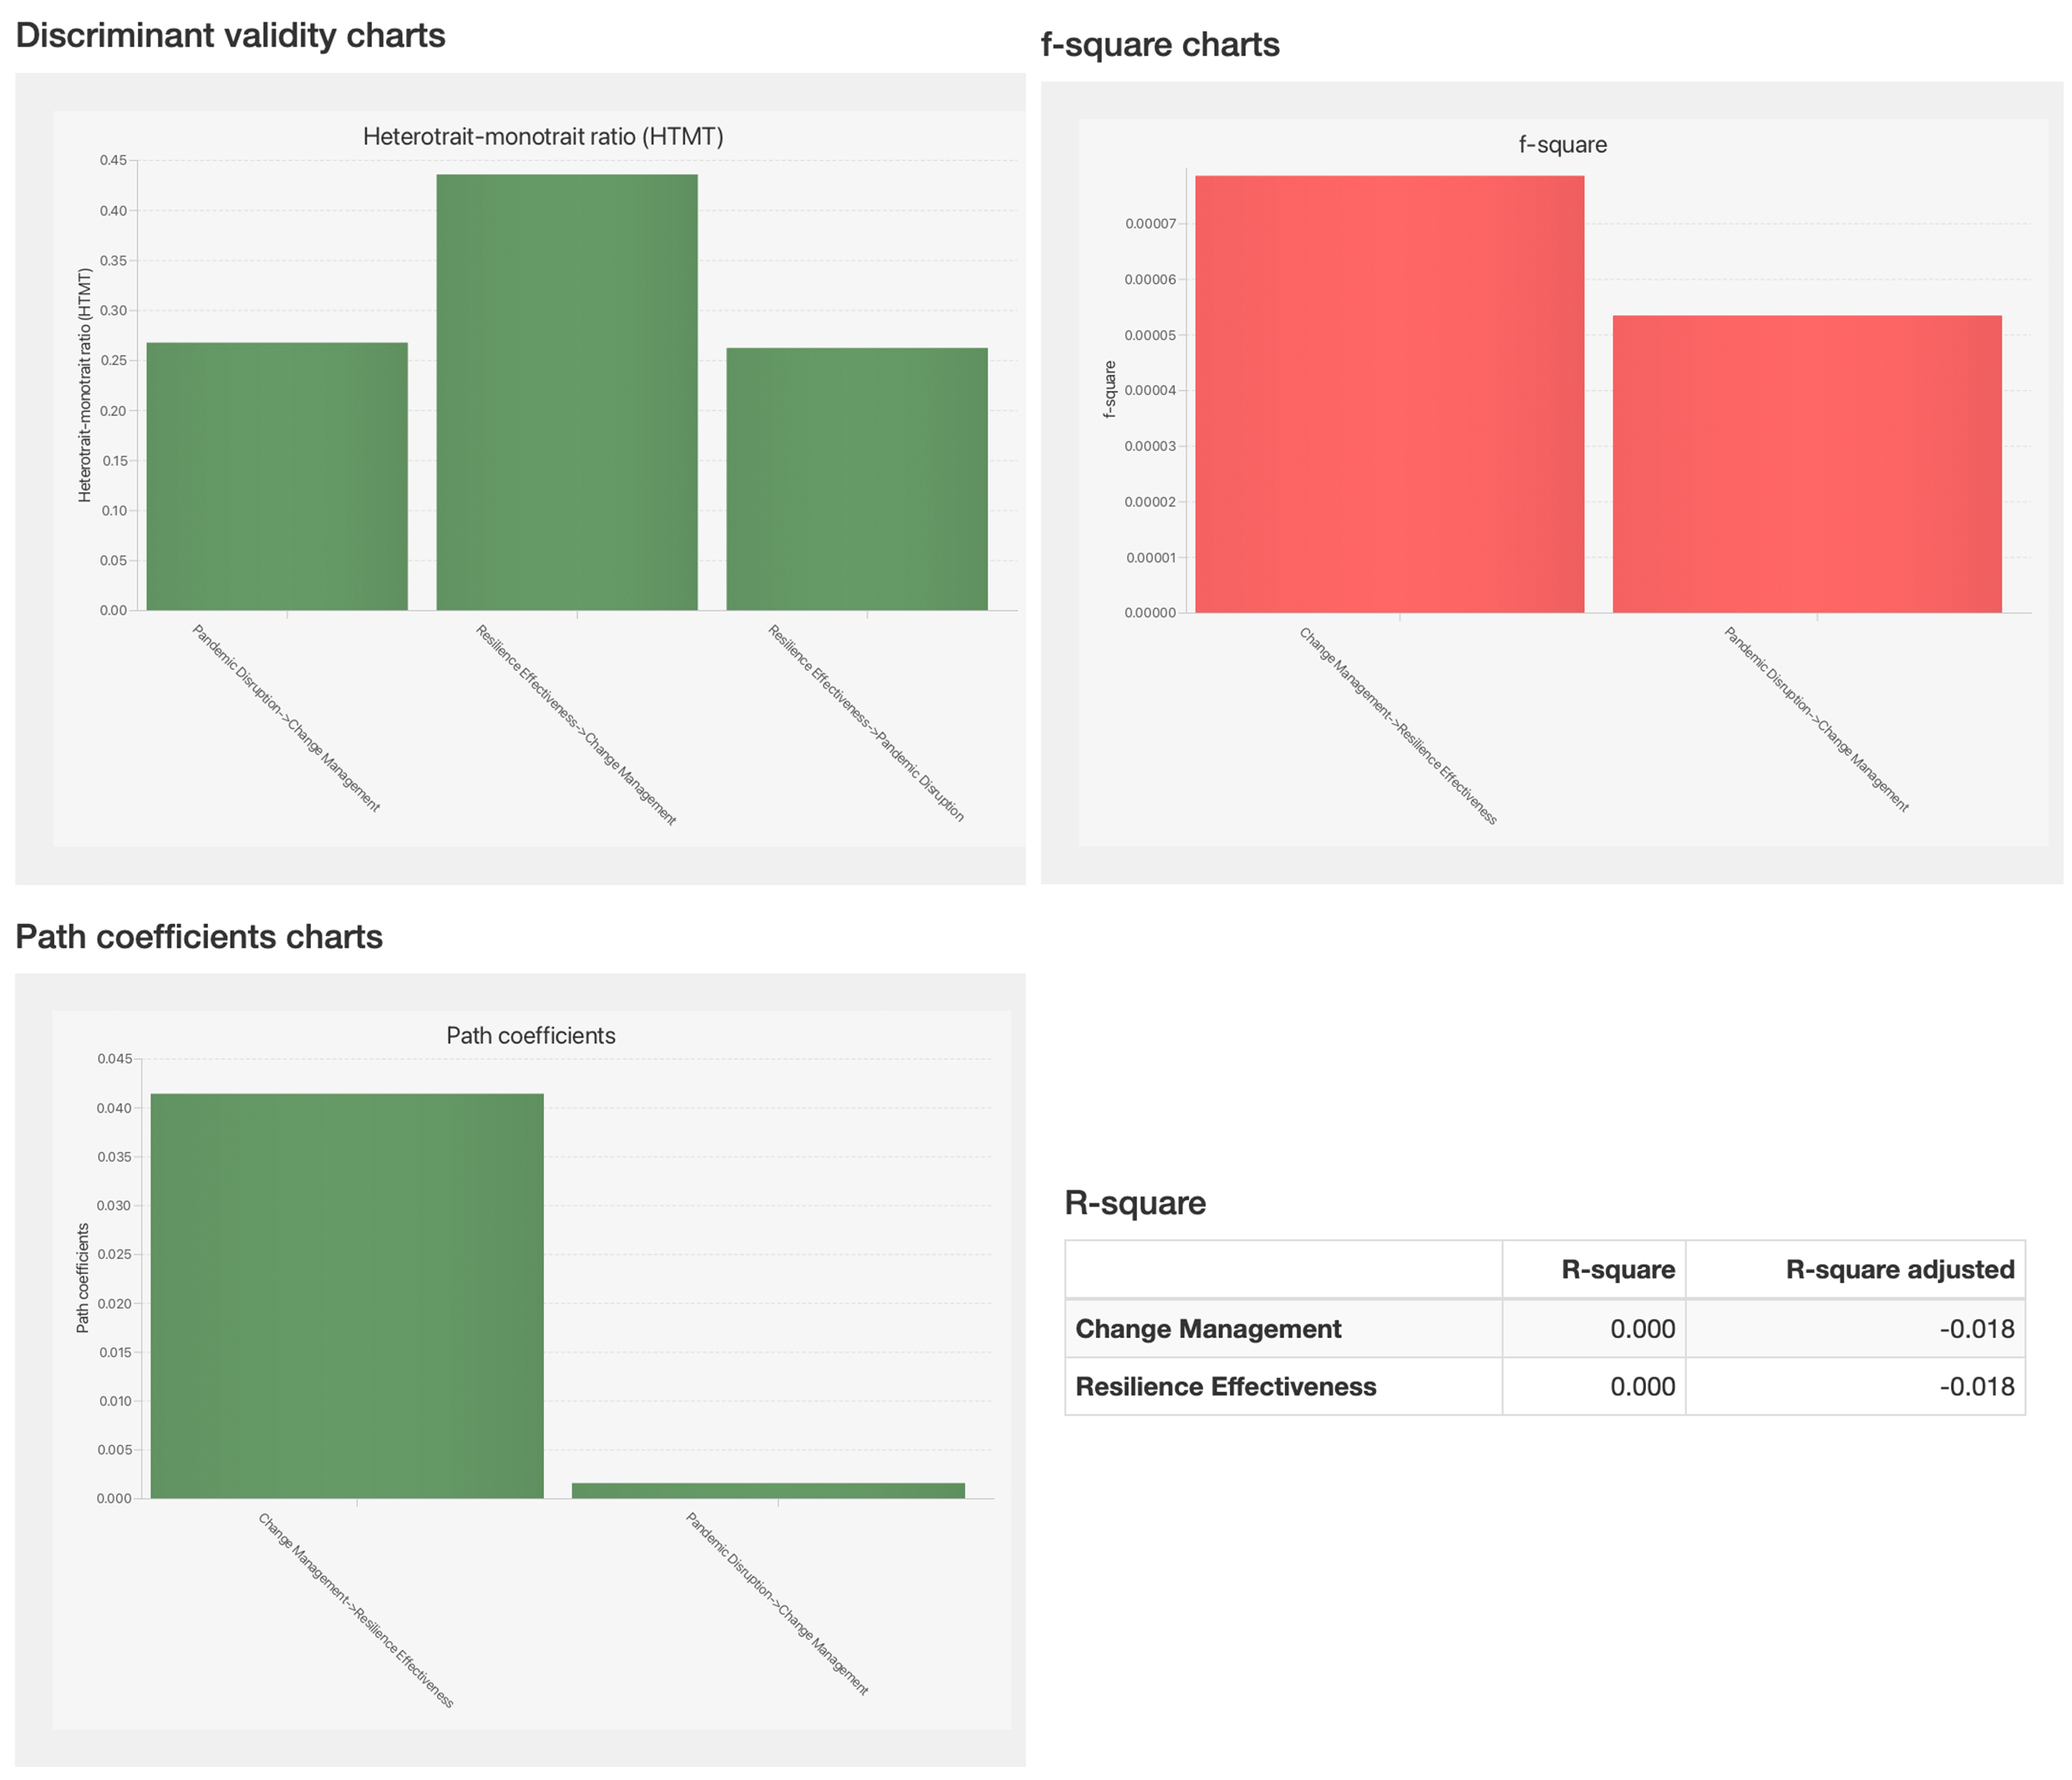
\includegraphics[width=1\textwidth]{figure/other_results.png}
  \caption{Other statistics from PLS-SEM analysis.}
  \label{fig:other_results}
\end{figure}

The results and analysis of PLS-SEM, as depicted in Figure \ref{fig:other_results}, offer further understanding of the relationships between the constructs of Pandemic Disruption, Change Management, and Resilience Effectiveness. The path coefficients chart confirms the previously discussed minimal impact, with the coefficient from Pandemic Disruption to Change Management being virtually zero (0.002), indicating a negligible direct effect. The slightly positive coefficient from Resilience Effectiveness to Change Management (0.041) suggests a weak but positive influence, implying that effective resilience strategies marginally contribute to change management efforts. The R-square values for both Change Management and Resilience Effectiveness are zero, indicating that the model does not explain any variance in these constructs, which may suggest either the lack of a strong relationship or limitations in the model's ability to capture the dynamics. The f-square values, though small, provide insight into the effect sizes, with Change Management to Resilience Effectiveness showing a slightly higher value compared to Pandemic Disruption to Change Management, indicating that resilience strategies have a somewhat more substantial influence on change management. The discriminant validity, assessed through the Heterotrait-Monotrait ratio (HTMT), indicates acceptable values below the threshold of 0.85, confirming that the constructs are distinct from each other. The SRMR (Standardized Root Mean Square Residual) values are 0.172 for the saturated model and 0.180 for the estimated model, both exceeding the recommended threshold of 0.08, suggesting a poor model fit and potential issues with the structural model specification. These results imply that while some relationships are weakly supported, the overall model does not adequately capture the variance and relationships between the constructs, indicating the need for model refinement or consideration of additional variables to better understand the dynamics at play.

Based on expert analysis and observation of our dataset, several factors have been identified that may explain why we were unable to establish strong correlations in our PLS-SEM analysis. Firstly, the lack of variability in the Change Management questions (CMQ5, CMQ6, CMQ8, CMQ9, CMQ10), where responses were predominantly '1' (Yes), significantly limits the statistical power of our analysis. The homogeneity in these responses means there is insufficient variation to explain the variance in dependent constructs, thereby hindering the detection of meaningful relationships. While the Pandemic Disruption variable (PDQ4) exhibited more variability, ranging from 0.8 to 5, its effectiveness in revealing correlations is compromised when paired with less variable indicators. Similarly, Resilience Effectiveness (REQ7) showed reasonable variability, ranging from 1.5 to 5, but the overall analysis suffers from the lack of diversity in binary responses. The binary nature and the high prevalence of a single response category diminish the ability of PLS-SEM to uncover underlying patterns, as significant paths are often established through variance explained by independent variables. The presence of potential ceiling effects, where binary indicators in the Change Management construct consistently hit the upper limit of their scale, further complicates the analysis by obscuring genuine relationships. This effect results in insufficient differentiation among responses, making it difficult to discern how changes in one variable relate to another. Lastly, the model configuration and theoretical considerations play a crucial role; our current model setup may not adequately capture the expected relationships if the theoretical assumptions are not perfectly aligned with the observed data. The predominance of 'yes' responses in the Change Management questions indicates that minor deviations might not statistically explain variations in Resilience Effectiveness, especially if the resilience question encompasses broader aspects of the pandemic's impact than anticipated. Consequently, while the results might indicate no correlation, it is also possible that due to the dataset's characteristics, existing correlations could not be established, highlighting the need for further refinement and consideration of additional variables.
















% \subsubsection{Purpose}
% Placeholder Text

% \subsubsection{Overview}
% Placeholder Text

% \subsection{Model Specification}
% Placeholder Text

% \subsubsection{Constructs and Measurement}
% Placeholder Text

% \subsubsection{Model Design}
% Placeholder Text

% \subsection{Evaluation of Measurement Model}
% Placeholder Text

% \subsubsection{Indicator Reality}
% Placeholder Text

% \subsubsection{Construct Reliability and Validity}
% \textbf{Internal Consistency Reliability}

% \textbf{Convergent Validity}

% \subsubsection{Discriminant Validity}

% \subsubsection{Summary}

% \subsection{Evaluation of Structural Model}

% \subsubsection{Path Analysis}
% \textbf{Path Coefficients}
% \textbf{Direct and Indirect Effects}

% \subsubsection{Model Fit}

% \subsubsection{R-Squared $(R^2)$ Values}

% \subsubsection{Effect Sizes $(f^2)$ Values}

% \subsection{Model Assessment and Validation}

% \subsubsection{Collinearity Statistics}

% \subsubsection{Robustness Checks}

% \subsection{Discussion of Findings}

% \subsubsection{Interpretation of Results}

% \subsubsection{Implications}

% \subsection{Limitations and Future Research Directions}

% \subsection{Conclusion}